\clearpage
\section{Details of Numerical Models for DEF Simulation}

\subsection{Introduction}

The exactly same model is used for DEF simulation in order to cross compare the cracking patterns and mechanical properties changes under ASR and DEF expansion.

\subsection{Geometry of Numerical Models}

The geometry of the models is exactly the same as models using in ASR simulation, which is in dimension of $100 \times 100 \times 100$ mm.

All materials properties are set to be exactly the same.

\subsection{Coarse Aggregate of Numerical Models}

To analysis the behavior of concrete with different coarse aggregate volume ratio, 15\% coarse aggregate model and 30\% coarse aggregate model (Figure \ref{skjdfhlk}) are built for simulation.

\begin{figure}[!h]
\centering
\begin{subfigure}{.5\textwidth}
  \centering
  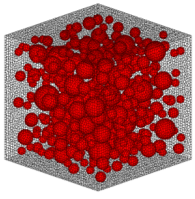
\includegraphics[width=.6\linewidth]{Files/Aggregate/A15.png}
  \caption{15\% Coarse Aggregate}

\end{subfigure}%
\begin{subfigure}{.5\textwidth}
  \centering
  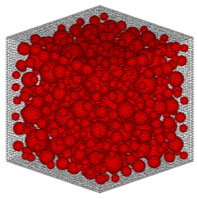
\includegraphics[width=.6\linewidth]{Files/Aggregate/A30.png}
  \caption{30\% Coarse Aggregate}
\end{subfigure}

\caption{Coarse Aggregate Percentage}
\label{skjdfhlk}
\end{figure}

\subsection{DEF Intensified Expansion Area of Numerical Models}

Since DEF is closely related to higher curing temperature, here we choose to intensified the expansion in center part of model.

Here we chooses 3 cases in different expansion intensified area. The Table \ref{table:DEF_X} is a list of cases simulated, illustration is presented in Figure \ref{fig:DEFffff_X}.

\begin{table}[ht!]
  \caption{DEF Intensified Expansion Area}
\centering
\begin{tabular}{||c c c||}
 \hline
 Case &  Expansion Intensified Depth[mm] &  Expansion Intensified Zone \\ [0.5ex]
 \hline\hline
 1 & 0 & $100 \times 100 \times 100$ mm \\
 2 & 12.5 & $75 \times 75 \times 75$ mm \\
 3 & 25 & $50 \times 50 \times 50$ mm \\ [0.5ex]
 \hline
\end{tabular}

\label{table:DEF_X}
\end{table}

\begin{figure}[ht]
\centering
    %*******
    \begin{subfigure}{.33\textwidth}
      \centering
      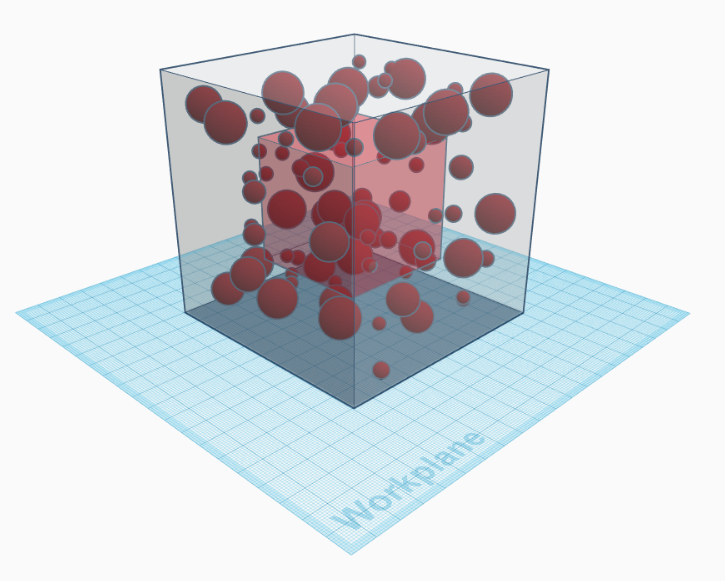
\includegraphics[width=.8\linewidth]{Files/DEF_X/X0_3d.png}
      \caption{Intensified  \\ $50 \times 50 \times 50$ mm Case}
    \end{subfigure}%
    %*******
    \begin{subfigure}{.33\textwidth}
      \centering
      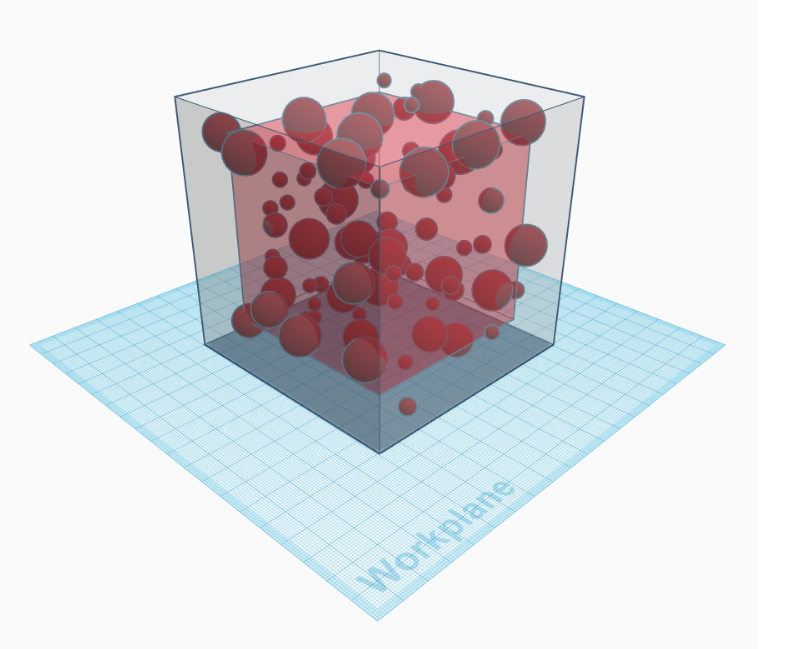
\includegraphics[width=.8\linewidth]{Files/DEF_X/X-5_3d.png}
      \caption{Intensified  \\ $75 \times 75 \times 75$ mm Case}
    \end{subfigure}%
    %*******
    \begin{subfigure}{.33\textwidth}
      \centering
      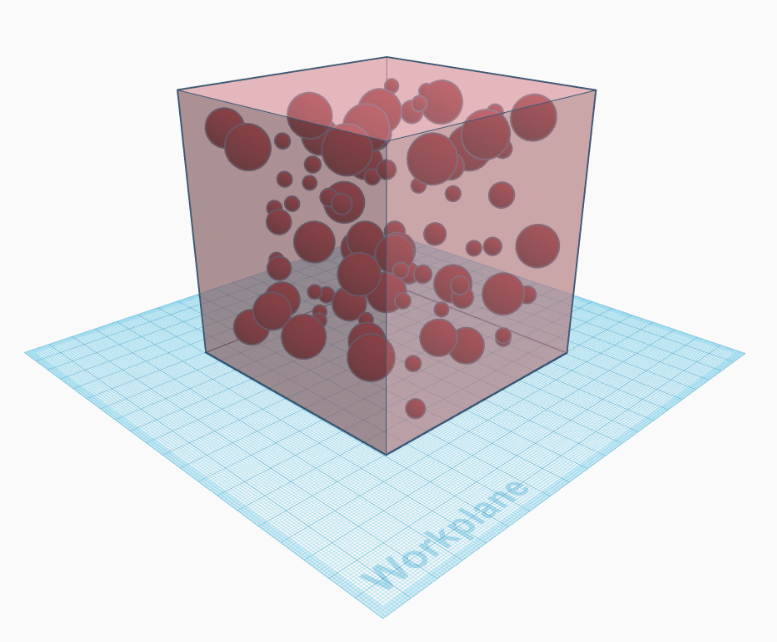
\includegraphics[width=.8\linewidth]{Files/DEF_X/X-1_3d.png}
      \caption{Intensified  \\ $100 \times 100 \times 100$ mm Case}
    \end{subfigure}
    %*******
    %*******
    \begin{subfigure}{.33\textwidth}
      \centering
      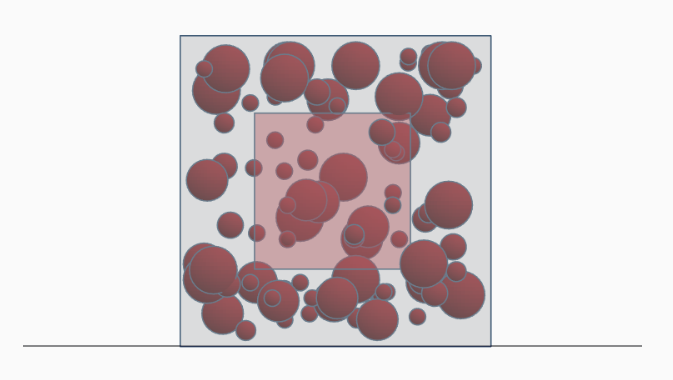
\includegraphics[width=.8\linewidth]{Files/DEF_X/X0_3ds.png}
      \caption{Intensified  \\ $50 \times 50 \times 50$ mm Case\\ Cross Section}
    \end{subfigure}%
    %*******
    \begin{subfigure}{.33\textwidth}
      \centering
      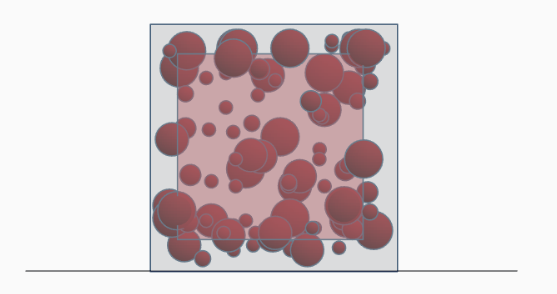
\includegraphics[width=.8\linewidth]{Files/DEF_X/X-5_3ds.png}
      \caption{Intensified \\  $75 \times 75 \times 75$ mm Case \\ Cross Section}
    \end{subfigure}%
    %*******
    \begin{subfigure}{.33\textwidth}
      \centering
      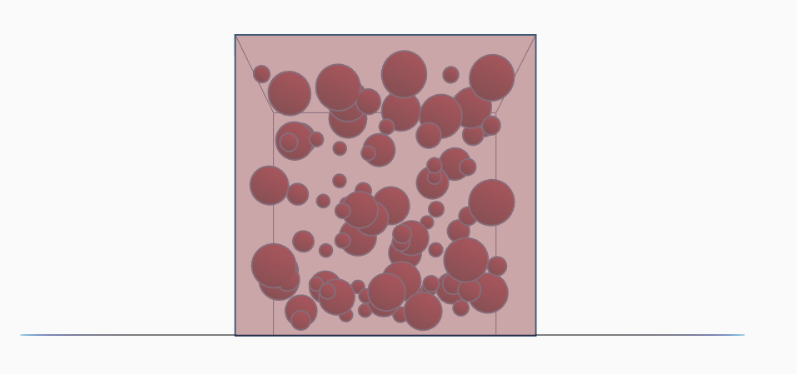
\includegraphics[width=.9\linewidth]{Files/DEF_X/X-1_3ds.png}
      \caption{Intensified  \\ $100 \times 100 \times 100$ mm Case\\ Cross Section}
    \end{subfigure}
    %*******
  \caption{DEF intensified part range}
  \label{fig:DEFffff_X}
\end{figure}

\subsection{Boundary Conditions}

\subsubsection{Boundary Condition During DEF Expansion}

Same as in ASR expansion, during DEF expansion, no confinements are added to the boundary elements. Models expanse freely in all directions.

\subsubsection{Boundary Conditions During Uni-axial Loading Test}

Same as in ASR expansion, Uni-axial Loading Test is applied with both fixed and free boundary conditions(Figure \ref{boundaaary}).

\begin{figure}[h!]
  \centering
  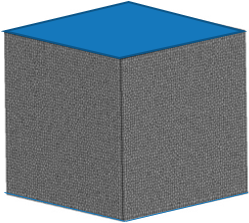
\includegraphics{Files/Background/LOAD.png}
  \caption{Top and Bottom Boundary in Loading}
  \label{boundaaary}
\end{figure}

In the case of fixed boundary condition, displacement in all directions are assumed as 0 at the bottom. Displacement in horizontal directions are all assumed as 0 at the top, and displacement in vertical direction is increased by 0.02 mm downward at each loading step.

In the case of free boundary condition, all boundary elements able to move freely in horizontal direction except 2 center elements in top and bottom are fixed in horizontal direction, to prevent the sliding of whole model during loading. Same as fixed boundary condition cases, displacement in vertical direction is increased by 0.02 mm downward at each loading step for top boundary elements.

Loading is applied until the maximum compressive strength is reached.
